\chapter{Abstract, italian}

\section*{Introduzione}

Fin dall'avvento dei primi calcolatori, l'ambito accademico scientifico ha
svolto un ruolo fondamentale nel guidare il progresso dai singoli mainframe ai
supercomputer.
In questi anni stiamo assistendo a una fase di transizione da un'infrastruttura
tradizionale di High-performance computing (HPC) al cloud computing
\cite{Surbiryala2019CloudCH}.
In questo elaborato, sarà esaminato uno dei componenti critici che
caratterizzano questa transizione, che potrebbe rappresentare il principale
collo di bottiglia nel porting dei codici per un ambiente HPC a questo nuovo
paradigma infrastrutturale: la \textit{Container Network Interface} (CNI).


\textit{"Cloud computing"} è un termine generico che comprende diverse soluzioni per
fornire servizi di calcolo su richiesta \cite{rajkumar2011}.
Pertanto, è necessario specificare maggiori dettagli per meglio delineare
l'ambiente in cui questo elaborato opera.
Per essere precisi, in relazione alla definizione proposta dal NIST
\cite{nistdef}, il \textit{cloud} preso in oggetto è un esempio di
\textit{"private cloud"}, dove l'infrastruttura è di possesso ed ad uso
esclusivo di una singola organizzazione.
Oltre all'infrastruttura fisica, sarà presentato Kubernetes come proposta di
\textit{"container orchestrator"}.
L'orchestratore, sempre in rispetto alla definizione NIST, agisce come
\textit{"Platform as a Service"} (PaaS) e le sue funzionalità sono state
completate con l'integrazione di software per il calcolo scientifico in modalità
\textit{"Software as a Service"} (SaaS).
Kubernetes condivide con i tradizionali job scheduler del mondo dell'HPC
(come ad esempio SLURM o PBS) molti aspetti della gestione delle risorse ma,
come sarà evidenziato nello sviluppo di questa tesi, da solo non è sufficiente
per essere usato come sosttuto. A tal proposito è possibile però estendere le
capacità di quetso orchestratore con dei plugin aggiuntivi per arrivare a
ottenere un prodotto, in termini di funzionalità, equivalente agli scheduler del
panorama HPC.


Un installazione di Kubernetes è infatti per certi aspetti molto simile ad un
nodo singolo in un ambiente di HPC, peoichè condivide lo stesso insieme di
applicativi Linux per la gestione delle risorse \cite{jain2023}. Tuttavia, nel
momento in cui si passa al calcolo \textit{distribuito}, è necessario aggiungere
alcuni componenti per garantire la scalabilità.
Il primo plugin che è necessario introdurre è il CNI già menzionato in
precedenza. Questo componente è responsabile della comunicazione tra nodi
diversi, aggiungendo tuttavia un overhead solitamente non riscontrato
nell'utilizzo degli approcci tradizionali di HPC.
Ne consegue che la scelta del CNI utilizzato (diverse alternative esistono),
rappresenta una delle decisioni più critiche quando si pianifica di installare
un infrastruttura di cloud computing che ha l'ambizione di proporsi come
alternativa all'HPC classico.
In questa tesi, esamineremo e confronteremo innanzitutto come diversi CNI
performano in diverse situazioni, passando dall'esecuzione di codici HPC
classici (con C ed MPI) fino a paradigmi di calcolo scientifico distribuito più
recenti, come la popolare libreria python Dask \cite{dask2015}, confrontando i
risultati ottenuti eseguendo gli stessi codici in un'infrastruttura HPC
all'avanguardia.

% Remove it?
%%%%%%%%%%%%%%%%%%%%%%%
 % Infine, mostreremo come integrare le nostre scoperte con il progetto open
 % source JupyterHub, una versione multiutente di Jupyter Notebook, per creare una
 % piattaforma funzionale e performante per il data science.
%%%%%%%%%%%%%%%%%%%%%%%


\section*{Metodologie}


Nel contesto del cloud computing, due tecnologie si sono affermate come standard
per lo sviluppo di applicazioni: macchine virtuali e i containers.
Una macchina virtuale (VM) è una rappresentazione a livello software di un
sistema informatico fisico (hardware) che consente alle applicazioni e ai
sistemi operativi di essere eseguiti in un ambiente separato e contenuto.
Questa tecnica si basa su un hypervisor, un programma che opera come
intermediario tra l'hardware fisico e i sistemi operativi delle macchine virtuali.
Il ruolo dell'hypervisor è quello di allocare risorse fisiche ed emulare un
ambiente hardware per la VM detta guest.
Ciò garantisce il massimo isolamento tra le VM poiché ogni VM è completamente
inconsapevole della presenza delle altre VM.
Tuttavia, l'hypervisor è anche la principale limitazione di questa soluzione
poiché questo livello intermedio introduce un overhead significativo e le
prestazioni delle VM sono inferiori a quelle di un sistema installato
direttamente nello stesso hardware.
Per questo motivo, le VM sono solitamente relegate a contesti in cui le
prestazioni non sono essenziali.

\noindent I containers, al contrario, operano secondo un principio diverso. Non
richiedono un hypervisor, ma condividono il kernel del sistema operativo host e
funzionano come processi isolati nello \textit{"user namespace"} sul sistema operativo
host. Ciò è reso possibile grazie ad alcune caratteristiche specifiche del
kernel Linux, ovvero: capabilities, namespaces e chroot.
Le capabilities consentono la restrizione dei privilegi del container, i
namespaces consentono l'isolamento delle risorse del container e la possibilità
di performare un \texttt{chroot} consente di modificare la root directory del
contenitore, creando di fatto un ambiente simile a una sandbox \cite{kerris2021,
  deochake2023}.
Il vantaggio principale dei containers sono le performance, poiché vengono eseguiti direttamente
sul sistema operativo host, senza l'overhead dell'hypervisor, consentendo al contenitore di avvicinarsi
alle prestazioni "bare metal" \cite{deochake2023}.
Per queste ragioni i container sono diventati lo standard de facto nel contesto delle soluzioni PaaS
e SaaS.
Considerando quanto affermato sino a questo punto, diventa assiomatico che la
soluzione proposta in questa tesi sia basata sulla containerizzazione.

Insieme al concetto di containerizzazione, gli orchestratori di container
dovrebbero essere menzionati per evitare di apparire anacronistici rispetto agli
standard moderni.
Questi strumenti sono responsabili della gestione del ciclo di vita dei
container, fornendo una piattaforma per automatizzare la distribuzione, il
ridimensionamento e il funzionamento dei container delle applicazioni su  un cluster.
Dal punto di vista dell'utente, l'orchestratore astrae l'infrastruttura
sottostante, consentendo di concentrarsi sull'applicazione piuttosto che
sull'hardware e fornendo un ambiente coerente per l'esecuzione
dell'applicazione.
Dal punto di vista infrastrutturale, l'orchestratore
gestisce la pianificazione dei container, l'allocazione delle risorse, il
ridimensionamento dell'applicazione e il monitoraggio dello stato
dell'applicazione, consentendo l'adozione dei container in un ambiente altamente
scalabile \cite{bookofkubernetes}.


Nel mondo open source, esiste una grande varietà di alternative per ciascuna
delle tecnologie menzionate sopra; per questa ragione è statno necessario
adottare criteri rigorosi per la selezione delle alternative adottate:
la popolarità del progetto, il livello di supporto della comunità che cura il
progetto, la completezza della documentazione disponibile e infine
l'integrabilità o meno con l'infrastruttura a  nostra disposizione nel cluster ORFEO.
Seguendo questi criteri, abbiamo scelto come sistema di orchestrazione dei
container \textit{Kubernetes} insiema al progetto \textit{helm}, come gestore di
pacchetti per Kubernetes.
Quest'ultimo copre la definizione, l'installazione e l'aggiornamento delle
applicazioni, mentre il primo è la parte fondamentale dell'infrastruttura cloud.
La decisione di utilizzare Kubernetes è stata determinata seguendo i criteri sopra menzionati
dal suo status di uno dei sistemi di orchestrazione dei container più popolari e
dal fatto che i principali provider cloud ne sostengono lo sviluppo.
Inoltre, ORFEO ha già un cluster Kubernetes in produzione che può essere
utilizzato come un solido esempio di come adottare alcune scelte tecnologiche
che possono garantire affidabilità a lungo termine.


In Kubernetes, i cluster multinodo sono organizzati sul concetto di  "nodo": una
parte fisica o virtuale del cluster.
Per consentire la comunicazione tra containers su nodi diversi, kublet (l'agente
Kubernetes) utilizza un  \textit{"Container Networ Interface Plugin"} (CNI
Plugin), ovvero un software che consente tale  comunicazione.
Questi plugin sono agiscono inserendo un'interfaccia di rete virtuale (ad
esempio, una coppia veth) nel network namespace del pod e apportando
tutte le modifiche necessarie alla configurazione di rete dell'host (ad esempio,
collegando tutti i vet a un bridge) per consentire al pod di  comunicare con
altri pod su altri nodi.
Alcuni dei plugin CNI più popolari e ampiamente utilizzati sono Flannel, Calico
e Cilium. Flannel, il più semplice, ha il vantaggio di funzionare in qualsiasi
situazione pronta all'uso;Calico offre un'ottima configurabilità e buone
prestazioni e consente la creazione di policy.
Infine, Cilium afferma di essere il "CNI nativo del cloud ad alte prestazioni".
Il cluster utilizzato, ORFEO, utilizza Calico al momento della stesura di
questo elaborato.


L'obiettivo principale di questo lavoro è mostrare le differenze tra i diversi
CNI e valutarne le prestazioni.
Per farlo, abbiamo impostato un'infrastruttura di test composta da tre nodi
(nodi di elaborazione connessi con Ethernet a 25 Gb) nella seguente configurazione:
un control plane e due nodi worker.
Tutti i nodi sono stati configurati con il sistema operativo (Fedora 40) appena
installato, utilizzano CRI-O com \textit{"Container runtime interface"}.
Oltre a questa configurazione, abbiamo installato diversi plugin CNI per i vari
test per valutare le prestazioni della rete.
L'idea è innanzitutto di testare come i vari CNI funzionano con la
configurazione predefinita di base e scegliere quella che porta alle migliori
prestazioni per la distribuzione futura, o se ciò non è possibile a causa di
vincoli di policy di rete, conoscere la perdita di prestazioni.


\noindent Il codice utilizzato per emulare un carico di lavoro HPC consiste
nell'eseguire il benchmark MPI OSU Micro-Benchmarks \cite{osudoc}. Per far ciò
si rende necessario aggiungere l'\textit{operatore} mpi all'infrastruttura
distribuita.
In Kubernetes, un operatore è un controller specifico per applicazione, pensato
per essere semplice e facile da usare che estende la funzionalità dell'API
Kubernetes per creare, configurare e gestire istanze di applicazioni complesse
con stato per conto di un utente \cite{bookofkubernetes}.
In pratica, durante il test, un pod viene generato in ciascuno dei nodi worker,
con ogni pod che esegue un container contenente il codice C degli OSU
Micro-Benchmarks e comunica con gli altri pod negli altri nodi.
In questo modo è possibile misurare latenza e bandwidth della rete per
determinare il miglior CNI plugin.


Performare un benchmark del workflow di un'infrastruttura di Cloud Computing si
può rivelare un compito decisamente impegnativo.
Innanzitutto, quale framework utilizzare? Si è deciso Dask perché meglio
siadatta al tipo di calcolo distribuito che si trova negli scenari moderni di
data science.
In secondo luogo, quale codice utilizzare come benchmark? Non è stato possibile
trovare un benchmark standard universalmente riconosciuto nella letteratura e
nelle varie comunità del progetto per giudicare  la bontà dell'infrastruttura su
cui è in esecuzione il codice.
A causa di questa assenza, abbiamo sviluppato un nuovo codice per soddisfare
questa esigenza.
Questo codice  esegue diverse operazioni, che coprono i casi d'uso più
diffusi nel settore scientifico. La prima sezione del codice simula la
manipolazione di array numerici multidimensionali, mentre la seconda fa lo
stesso ma utilizzando i dataframes come oggetti presi in esame.
La valutazione si basa sul concetto di "scalabilità debole" \cite{Hager2010}.
Questo significa che man mano che aumenta il numero di unità di calcolo (nel
caso specifico, core), il carico di lavoro globale aumenta, consentendo a
ciascuna unità di gestire un compito costante.
Nel caso ideale di scalabilità perfetta, il tempo dovrebbe rimanere costante.
Allo stesso tempo, la velocità delle operazioni al secondo eseguite (MB
elaborati al secondo) dovrebbe dipendere linearmente dal numero di core
utilizzati.

\section*{Risultati principali}

Innanzitutto una premessa importante per la sezione seguente: con l'espressione
"bare metal" si intende l'hardware fisico dei nodi nella partizione THIN del
cluster ORFEO, composto da macchine dotate di due Intel Xeon Gold 6126, 768 GiB
di RAM e, per questo studio, una scheda di rete da 25 Gb. Nel caso di Kubernetes
la configurazione hardware è la stessa del bare metal.
In questo secondo caso, infatti, sono stati utilizzati 3 nodi THIN per creare un
cluster Kubernetes, composto da un control plane e due nodi ``worker''.

Come accennato nella sezione metodologica, la prima valutazione si è incentrata
nel valutare le prestazioni di rete.
In particolare, la latenza e la bandwidth della rete sono state misurate per
determinare quale dei plugin CNI considerati abbia le migliori prestazioni.
L'esperimento è stato condotto per valutare sia la latenza minima che la
badnwidth massima raggiungibile dalla rete.
Poiché tutte le funzionalità che rendono Kubernetes una soluzione cisì
desiderabile richiedono che il piano di controllo interagisca con i pod che
amministra e la connessione tra i pod viene ottenuta collegando loro
un'interfaccia di rete virtuale, si prevede che il plugin CNI avrà un impatto
significativo sulle prestazioni di rete.

Dai dati presentati nella Figura \ref{fig:summary-osu_it}, è evidente che il
layer appena introdotto aggiunge una latenza sostanziale alla comunicazione.
La degradazione delle performance dipende fortemente dal plugin e varia da circa
1,79 a 3,25 volte rispetto al caso ``bare metal'' preso come baseline.
Tra i plugin studiati, visti i risultati ottenuti, Cilium si presenta come
l'alternativa migliore, almeno con le configurazioni di default utilizzate.
Queste maggiori prestazioni sono con gran probabilità dovute all'adozione del
nuovo dataplane eBPF che evita alcune elaborazioni del pacchetto di rete da
parte del netfilter.
 Al secondo posto c'è Calico, che, con la configurazione standard,
si comporta in modo simile all'ultimo Flannel.
Entrambe le soluzioni sono probabilmente ostacolate dall'incapsulamento richiesto nel
passaggio VXLAN su cui si basano (Flannel) e per l'utilizzo di iptables per le
funzioni di loadbalancing (Calico).
Al contarario, quando si prende come riferimento la bandwidth, Flannel è quello
che tra i vari candidati è riuscito a riportare i risultati più elevati nelle
misuraioni.
Tuttavia, in questo secondo caso, la differenza tra i plugin è
quasi trascurabile.
Il valore raggiunto alla convergenza è probabilmente dettato da
limiti interni in atto per garantire un uso equo delle risorse, come la
larghezza di banda, in scenari in cui l'obiettivo principale è garantire a
ciascun pod una discreta quantità di traffico.
Concentrandoci sulla seconda colonna, vediamo come la comunicazione pod-to-pod
venga rallentata e l'overhead introdotto dal software stack di kubernetes sia
estremamente impattante.

\begin{figure}
  \centering
  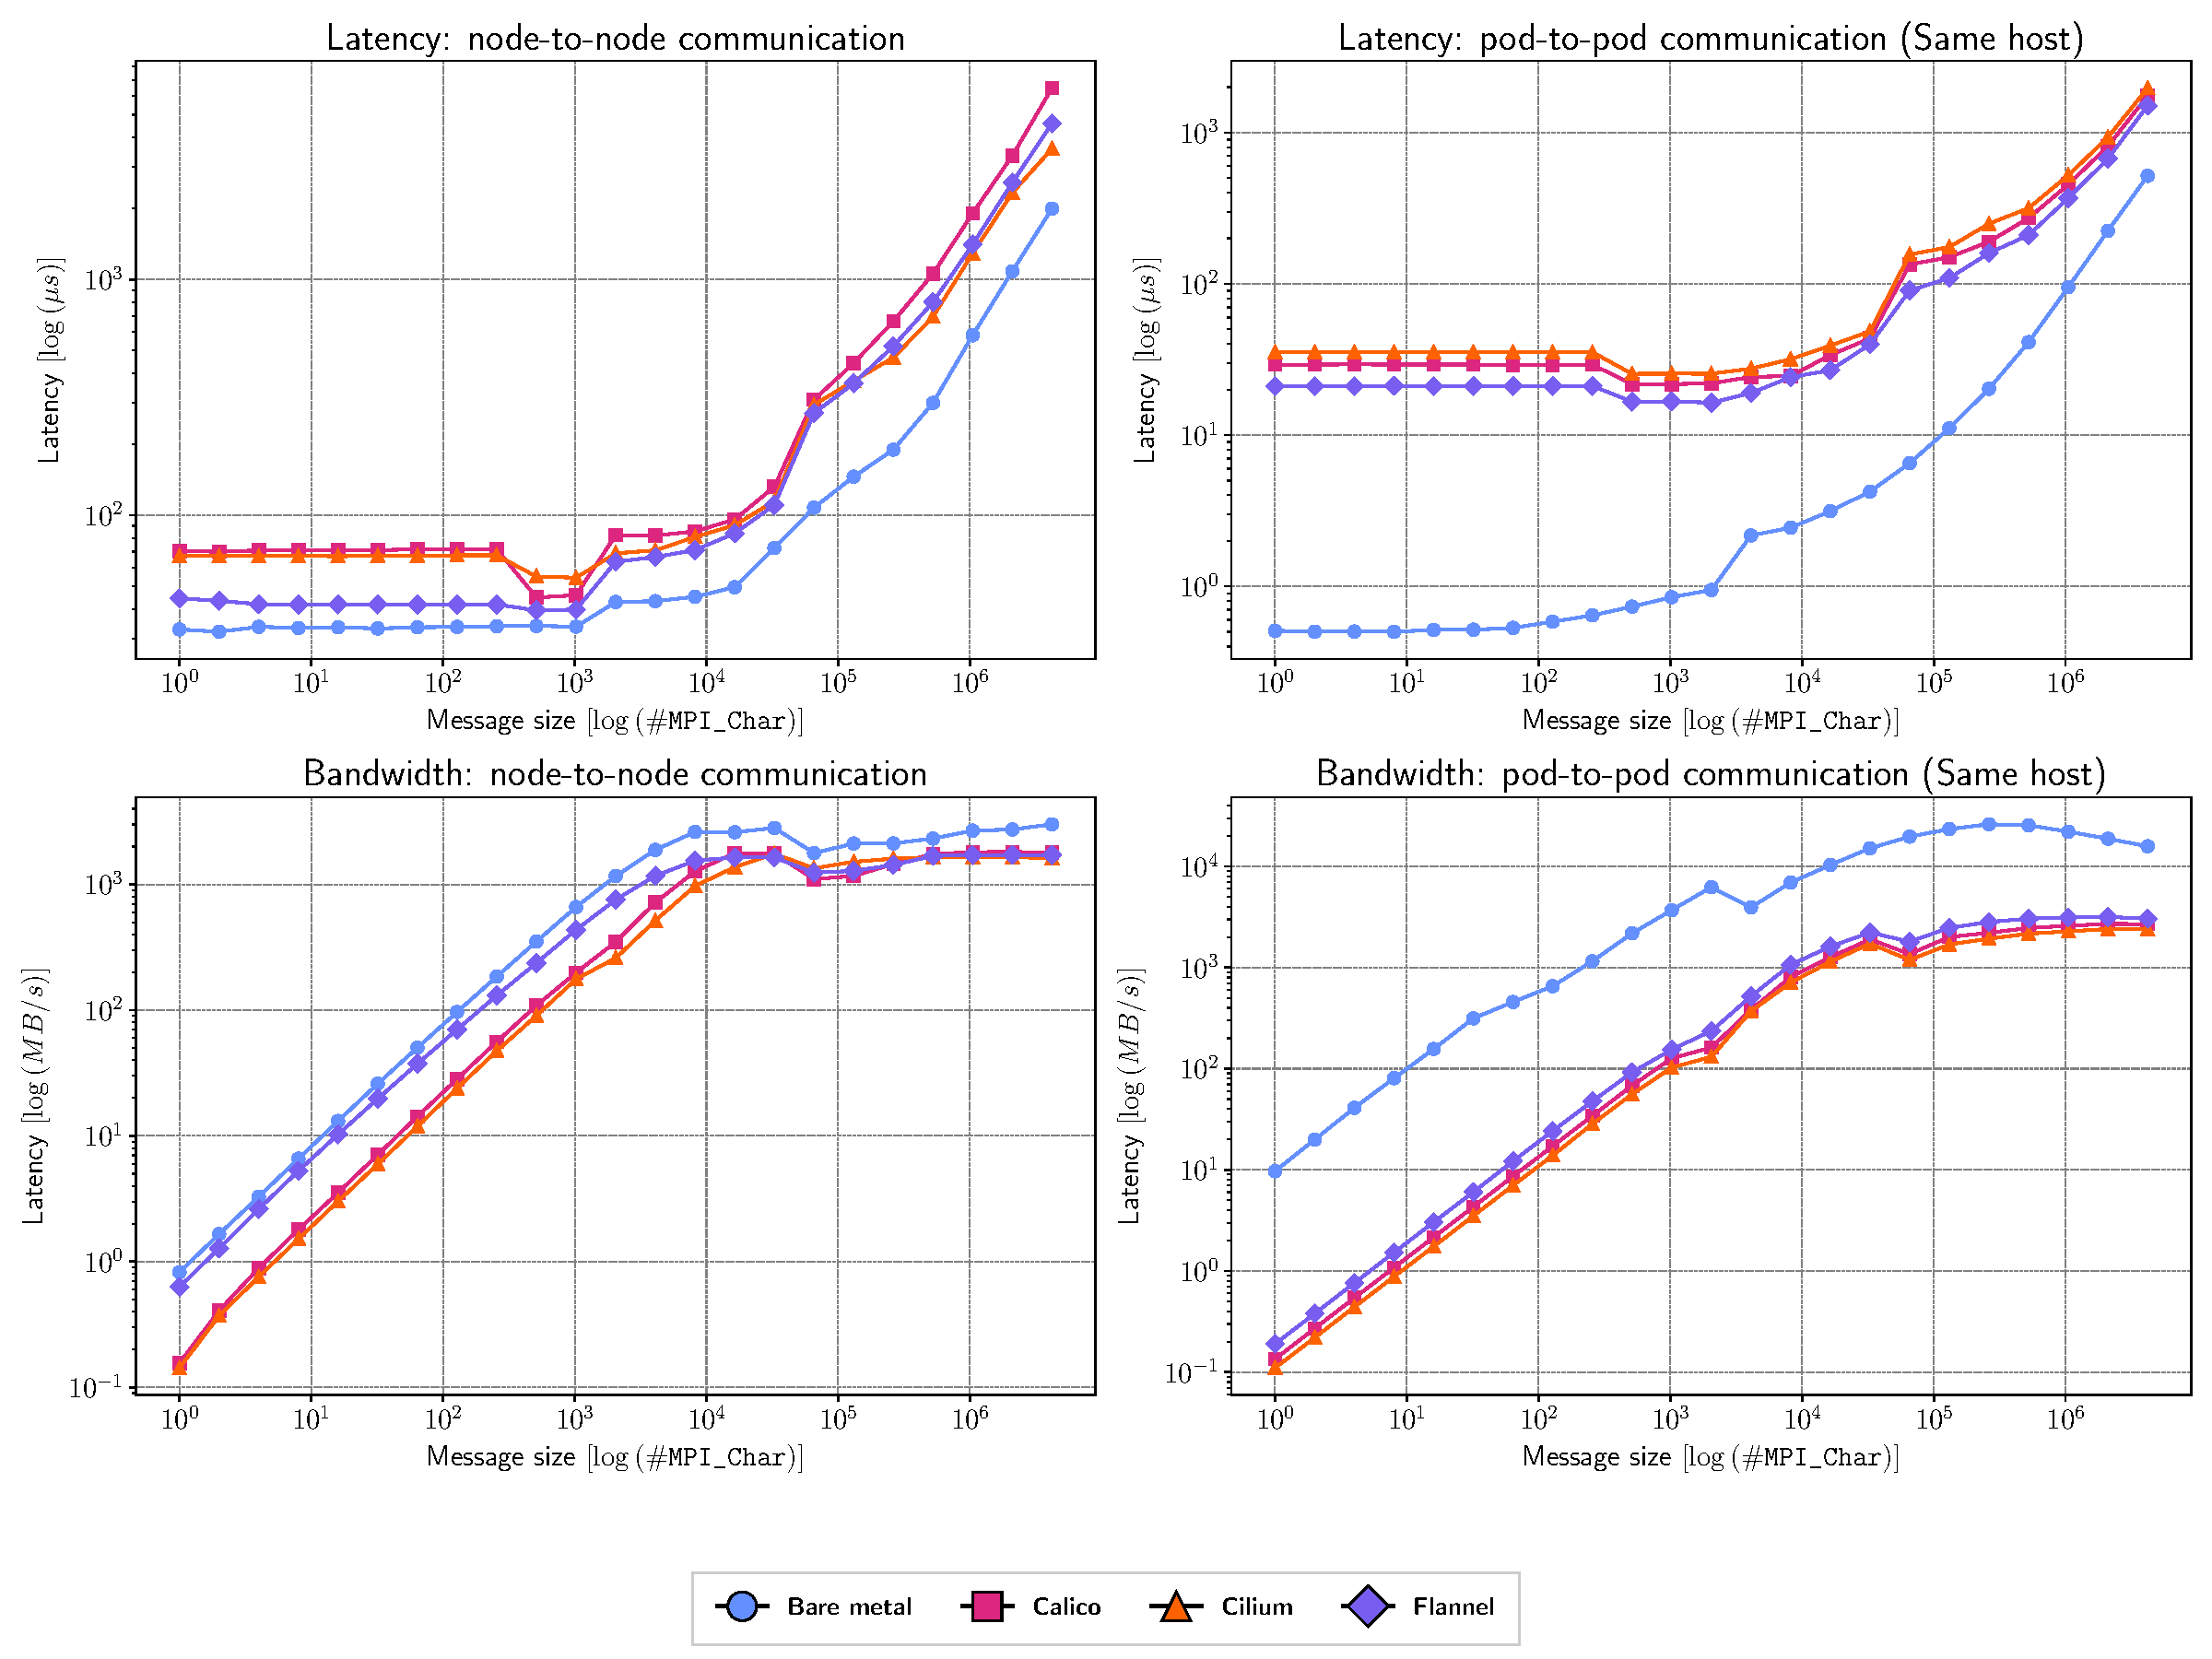
\includegraphics[width=\textwidth]{img/abstract/summary-osu}
  \caption{Risultati di Osu Micro-Benchmarks. La riga superiore mostra la
    latenza registrata (più basso il valore, meglio è) per diversi CNI in
    funzione della dimensione del messaggio MPI mandato e ricevuto.
    La riga inferiore mostra l'andamento della bandwidth (valori più alti sono
    migliori) per lo stesso set di configurazioni, sempre al variare della
    dimensione del messaggio trasmesso.
    La prima colonna mostra il risultato nella comunicazione da nodo a nodo
    mentre la seconda è il risultato della comunicazione pod-to-pod nello stesso
    nodo confrontato con i processi mpi sullo stesso dispositivo nel caso bare metal.
    Tutti i benchmark sono stati eseguiti 30 volte ed è quindi stata considerata
    la media di tutte le misurazioni.}
    \label{fig:summary-osu_it}
\end{figure}

Una volta stabilito che il plugin cilium CNI era la scelta più allettante,
il passo successivo è stato valutare le prestazioni dell'infrastruttura su cui il
codice è in esecuzione in un tipico carico di lavoro simulando operazioni
comunemente svolte nell'ambito dell data science.

Per fare questo è stato utilizzato il Dask Operator per Kubernetes.
Il vantaggio netto di questa scelta è che in questo modo lo stesso codice può
essere riprodotta in un'infrastruttura basata su Slurm e su Kubernetes allo
stesso modo.
Questa possibilità consente un confronto significativo tra test bare metal e
Kubernetes.
Il Dask Operator è un operatore Kubernetes che gestisce i cluster Dask.
Rimuovendo l'astrazione Kubernetes, è possibile generare un Dask client che
interagisce con SLURM per creare un oggetto "cluster", una raccolta di oggetti "worker".
Questi worker sono l'equivalente dei worker pod nell'infrastruttura Kubernetes,
ognuno dei quali è un processo separato con una quantità fissa di risorse assegnate.
In questo test, abbiamo iniziato con un singolo worker con un core e tutta la
RAM disponibile e abbiamo aumentato progressivamente il numero totale di core (e
worker quando il numero di core superava i 24 disponibili sui nodi THIN) per
valutare la scalabilità debole.


I seguenti risultati possono essere utilizzati per confrontare le prestazioni
delle due infrastrutture e per valutare la scalabilità del codice nel
cluster Kubernetes, dimostrando che l'implementazione cloud-based
del cluster può scalare in modo efficace quanto quella bare metal.
La figura \ref{fig:summary-dask_it}) mostra i risultati della
valutazione di alcune delle operazioni più comuni eseguite sugli array:



\begin{figure}
  \centering
  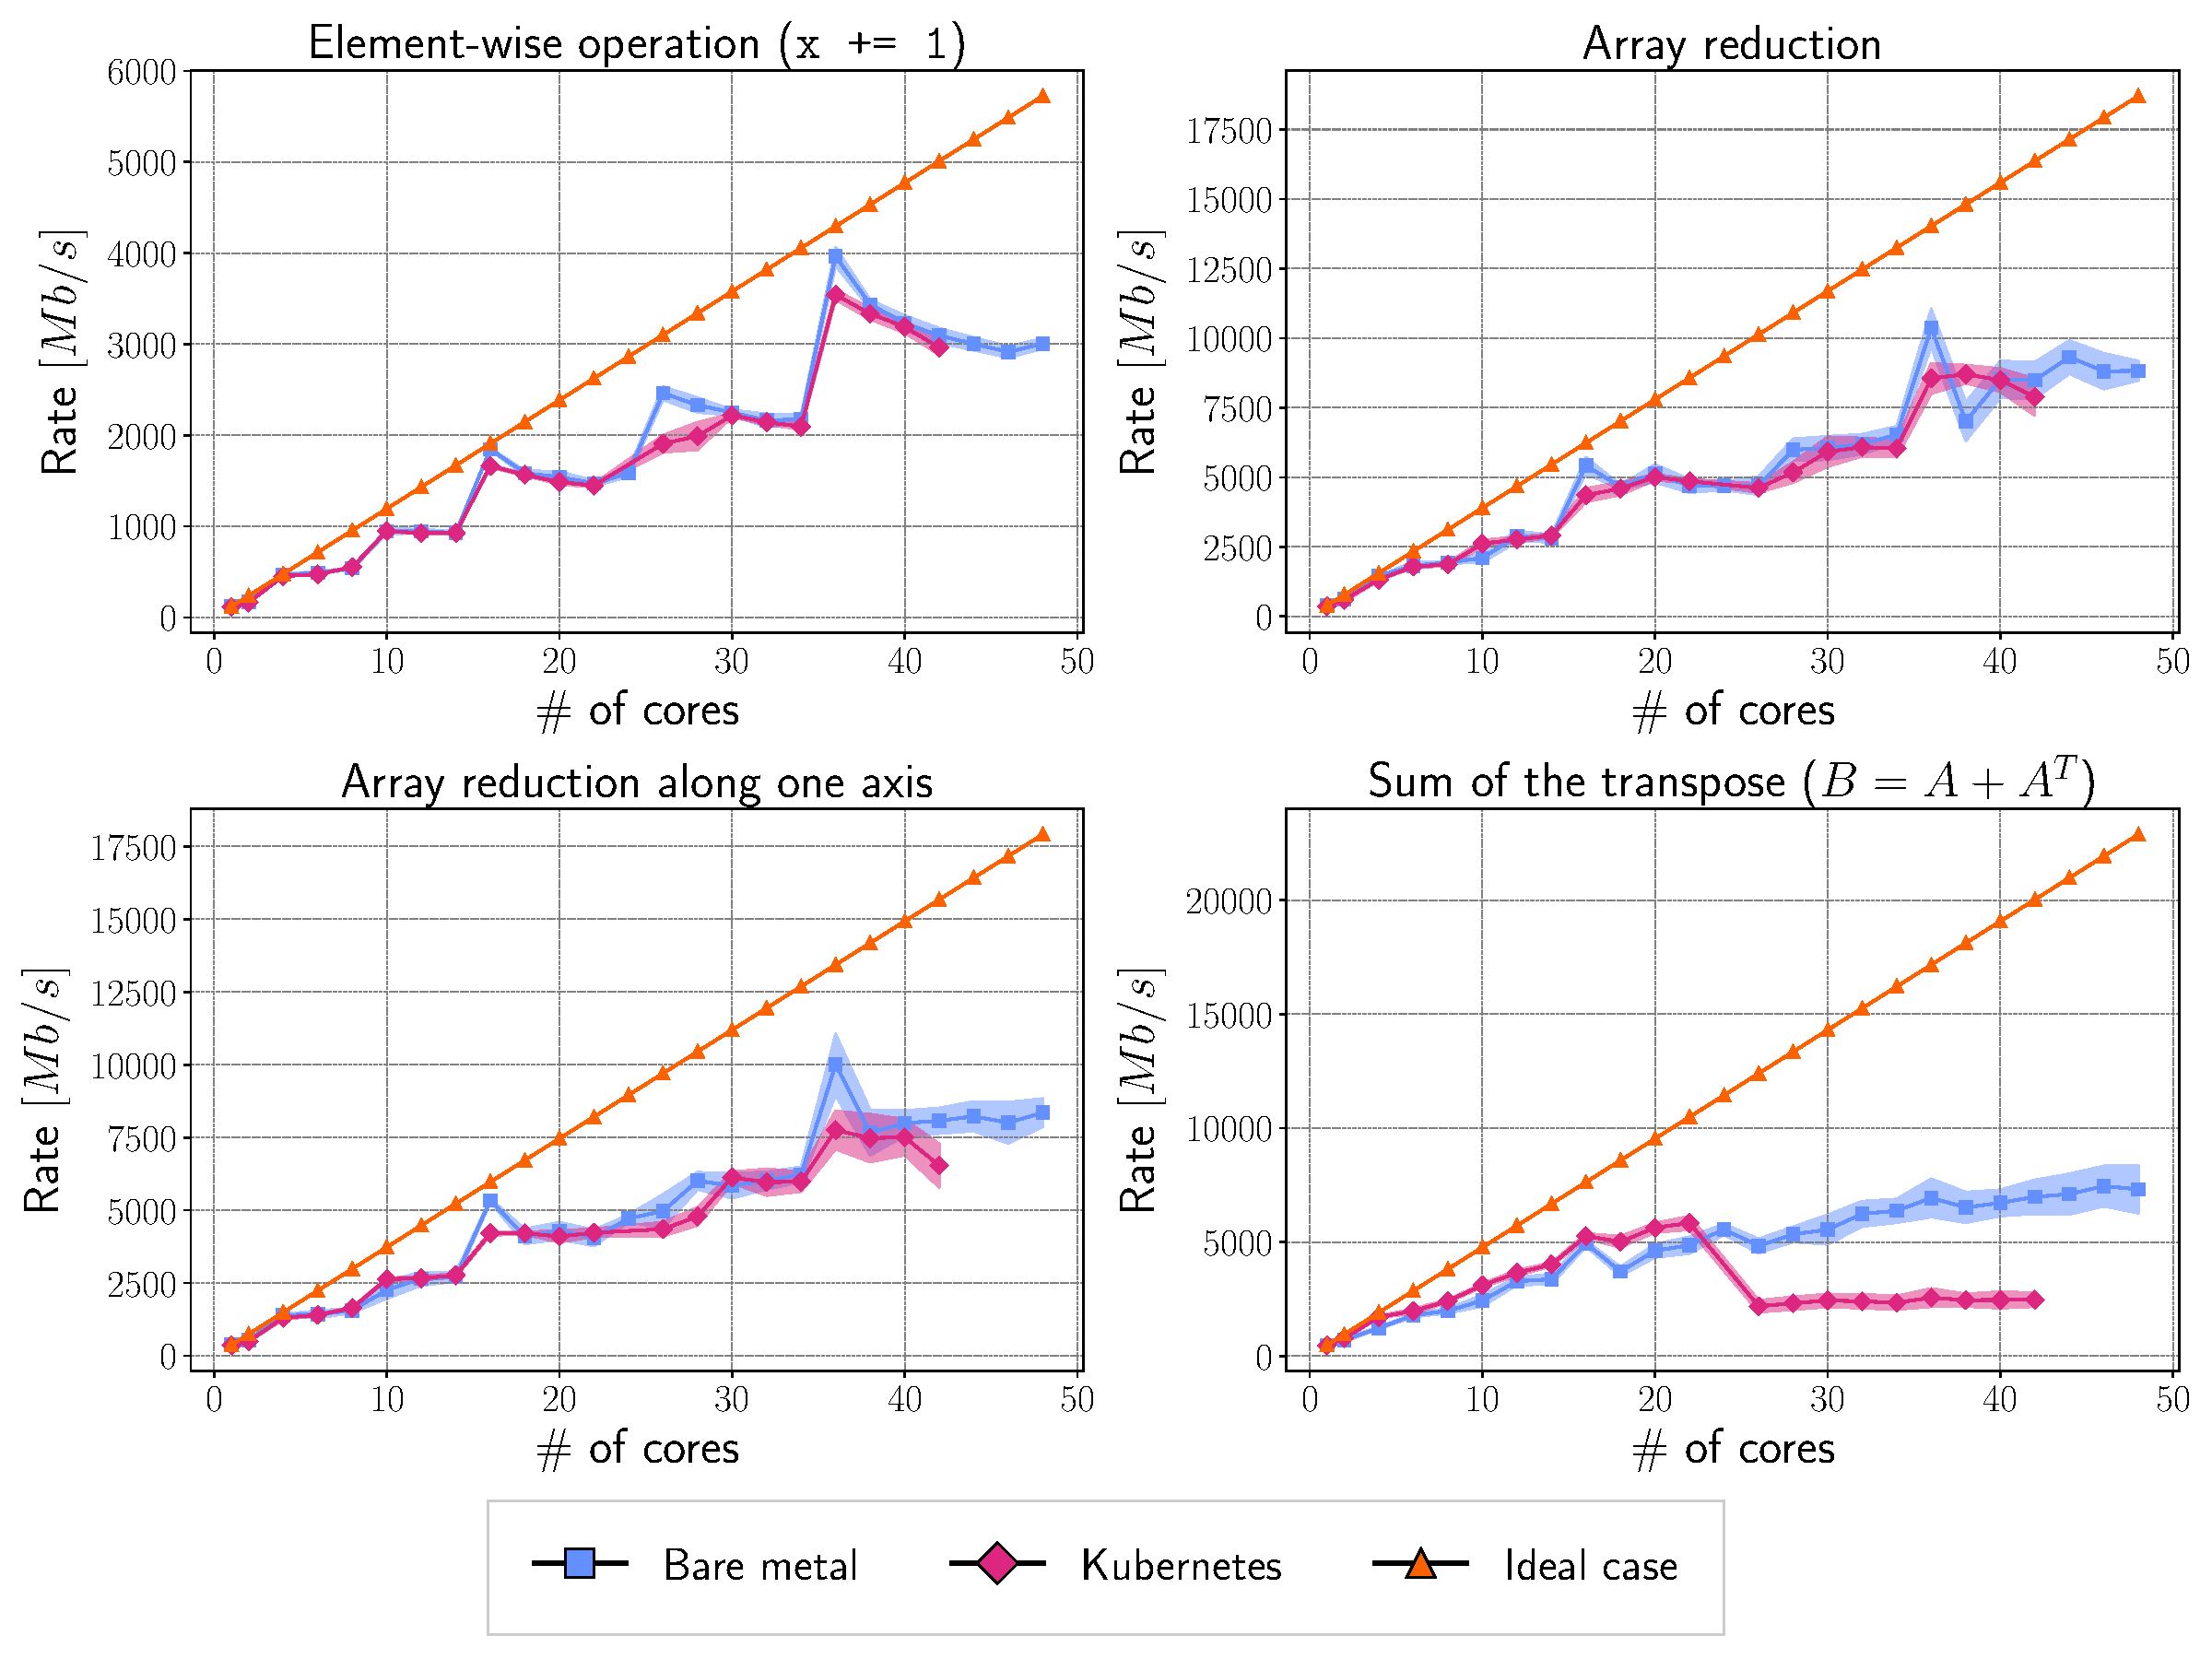
\includegraphics[width=\textwidth]{img/abstract/summary-dask}
  \caption{Risultato della valutazione delle prestazioni di Dask per alcune
    delle operazioni più comuni applicate agli array.
    Ogni benchmark è stato eseguito 30 volte e il valore medio è stato
    considerato.
    Questi risultati, in particolare, sono stati ottenuti considerando array
    bidimensionali.}
  \label{fig:summary-dask_it}
\end{figure}

Da questi risultati, la scalabilità del codice nell'impostazione Kubernetes proposta è
comparabile a quella ottenuta nella valutazione bare metal, con l'unica
eccezione degna di nota di problem ``communication bounded'' come nell'esempio
riportato della somma della matrice con la sua trasposta.
Questo è un risultato promettente, poiché mostra che la soluzione proposta può
sfruttare appieno le risorse del cluster, consentendo agli utenti di eseguire
calcoli paralleli.
I risultati hanno evidenziato alcune critiche nelle attività che richiedono molta
comunicazione, ma a parte questo, il cluster Kubernetes può essere una valida
alternativa all'infrastruttura HPC tradizionale poiché le prestazioni sono
assolutamente paragonabili a quelle bare metal.


\section*{Conlcusioni}

In questo lavoro, abbiamo analizzato la complessità di un'infrastruttura Cloud
atta a eseguire tasks tipiche dei server HPC, individuando il componente chiave
che agisce da collo di bottiglia quando si tenta di eseguire attività
impegnative: il networking.
Dopo aver sviluppato l'infrastruttura e discusso i suoi vantaggi, ci siamo
concentrati sul networking.
Qui, abbiamo confrontato la latenza e le prestazioni di larghezza di banda di
diverse CNI per l'infrastruttura Kubernetes.
Il risultato principale è che quando si tenta di parallelizzare il codice
utilizzando mpi, l'installazione predefinita di Cilium, grazie al dataplane
ebpf, supera tutte le altre soluzioni.
Questo vantaggio sembra diventare marginale quando abbandoniamo mpi a framework
di parallelizzazione più moderni, come Dask, utilizzati dalla comunità di data
science.
Tuttavia, Cillium è ancora incommensurabilmente più lento della velocità
prevista su una normale infrastruttura HPC in cui MPI può sfruttare tutte le
funzionalità del kernel e un'infrastruttura Infiniband.
Per risolvere questo problema, una possibilità è quella di estendere il test
alla CNI Mellanox. Inoltre, usare Multus per distribuire più di una CNI
contemporaneamente potrebbe consentire l'utilizzo di più canali di rete,
combinando potenzialmente sia Ethernet che InfiniBand, migliorando così le
prestazioni complessive della rete.
Come passo successivo, aggiungeremo un'interfaccia intuitiva (JupyterHUB) che
consentirà agli utenti di sfruttare facilmente tutti i vantaggi che la soluzione
Kubernetes comporta, come la standardizzazione e una maggiore portabilità del
codice, l'auto-scalabilità delle risorse richieste e, in generale, una maggiore
flessibilità.
